\section{Identification}

    As has hopefully been demonstrated, studies of orphan genes and
    phylostratigraphy can be very illuminating. However, there are many
    problems to consider.

    To really prove a gene is a de novo orphan: 1) prove that it is not present
    in other lineages 2) prove is is transcribed in some context 3) prove that
    it is translated.

\subsection{sORF}

  Short ORFs (sORF) \cite{kageyama_coding_2011}.

  Non-specific translation is common, as xanthicly reviewed here \cite{wilusz_long_2009}.  

  What constitutes evidence of functionality?

  Differential expression under differing conditions? This could just mean that
  the regulatory elements you have by chance are acted on by some other agent
  that is differentially expressed under the condition.

  Tissue specific expression? This could go either way. One could argue that
  since it is tissue specific, it must play some role in the development of that
  tissue. Another could argue that since it is tissue specific, it is probably
  under a simplistic regulatory paradigm (since broad exression actually requires
  more regulatory elemetns).

  Regulation during development? As above, all this means is that the possibly
  chance regulatory elements happen to be related to particular developmental
  stages.

  Association with disease? Same as above.

  What would constitute evidence of function? Concinnity of regulatory elements:
  multiple, independent pieces working toward a common end. For a coding
  sequence, any apparent influence of the amino acid meaning of the codons would
  be sign of functionality.

  Perhaps a better question would be, what would a non-functional ncRNA look
  like? Would it be expected to be expressed equally in all tissues and under all
  conditions? What is our null model?

  Many sORFs have been found in yeast \cite{kastenmayer_functional_2006}, they
  suggest ~5\% of genes in all species are sORFs ($<100$ aa). Many of these are
  conserved (not orphan).

  Hanada et al. developed an extensive pipeline for annotating sORFs
  \cite{hanada_large_2007}, which included analysis of nucleotide compostiion
  (codon usage and amino acid preferences) and, for those with detectable
  homologs, level of purifying selection.

  \begin{figure}[h!] \centering
      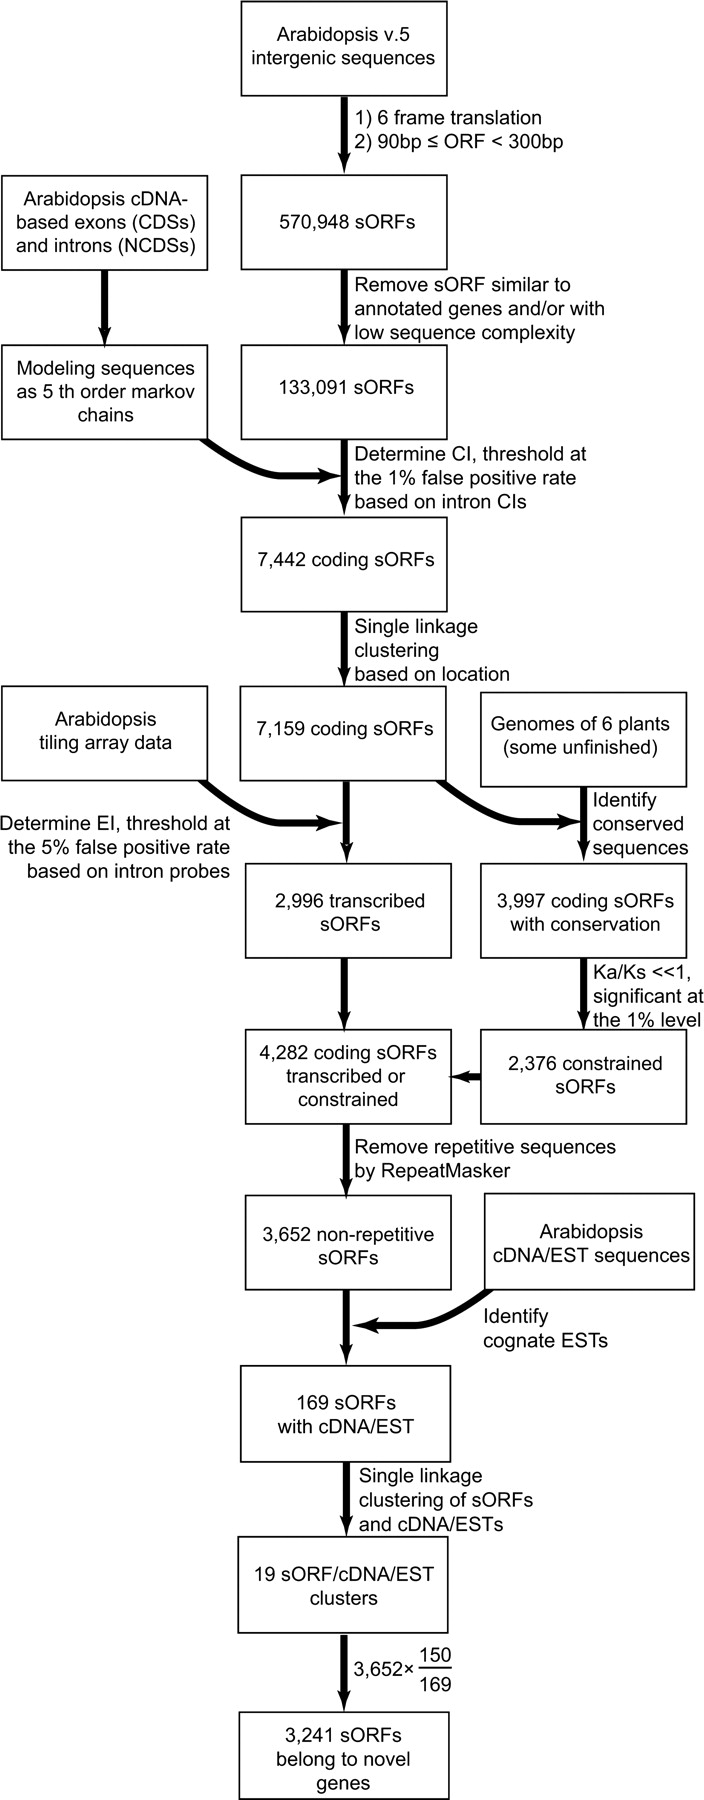
\includegraphics[height=0.5\textheight]{hanada-2007-fig1}
      \caption{hanada (2007) \cite{hanada_large_2007}}
  \end{figure}
  \FloatBarrier

\subsection{General notes}
Skovgaard suggested in 2001 that what we now would likely consider orphans
were non-functional ORFs, i.e. annotational artefacts
\cite{skovgaard_total_2001}. It is a quite good paper from the pre-RNA-seq
world.

Wilson (2007) \cite{wilson_large-scale_2007} proposes a Quality Index for
Predicted Proteins (QIPP) measure to predict which ORFs appear to be real
proteins. QIPP uses 5 criteria:

\begin{description}
    \item[Length]

    \item[Complexity] Sequence complexity, as calculated by SEG.

    \item[Cost]The metabolic cost of producing an amino acid. At least in
        bacteria, selection seems to favor amino acids that are
        metabolically less expensive. So neutrally evolving proteins should
        have higher costs on average.

    \item[GC Composition]

    \item[Neighborhood Distribution]Average of the number of genomes with
        homologues to the 5 genes flanking either side of a gene.
\end{description}


\subsection{BLAST}

PSI-BLAST traces motifs. There is the danger, however that it can trace
convergent evolution, jumping to new gene families. 

Use of several more advanced methods (PSI-BLAST, HHblits
\cite{remmert_hhblits:_2011}, HHpred \cite{hildebrand_fast_2009}, and some
manual shit) allowed identification of more distant homologs in $~25\%$ of
viral orphans \cite{kuchibhatla_powerful_2013}. Care should be taken however in
the interpretation of the results, especially with HHpred, since these may trace
convergent evolution.

\subsection{Phylostratigraphy}

What are we actually finding when we do phylostratigraphy? The ``founder
genes''? This is only true if these founders are de novo.

We want to find the de novo founder genes.

\subsection{Orphan Prediction}

Every phylostratigraphic analysis uses homology. There are many choices that
must be made: which homology algorithm, substitution matrix, gap penalties,
homology score cutoffs, whether to mask complexity (and which masking algorithm
and parameters to use), and what databases to search. Homology can be
augmented. For example, some researchers only count a match as a homolog if
query coverage exceeds some threshold. Augmenting with synteny is very
powerful, but also conservative and requires good genomes. The most certain way
to identify an orphan is by coupling homology and synteny. It is the gold
standard, the way to build test sets. However all predictions are contingent on
the accuracy of the genome annotations.

\subsection{Annotation}
\subsubsection{General issues}

  Here is a general, practical review of the annotation process written Yandell
  by the maker of MAKER \cite{yandell_beginners_2012}. There is a bit of fishy
  math in the paper, for example the assertion that if the ND50 is greater than
  the median gene length, then roughly 50\% of the genes will appear on a
  single scaffold.
  
  Yandell emphasizes the importance of repeat masking, reasoning that failing
  to do so can result in transposon ORFs being identified as coding genes or
  their exons being incorporated into gene models. However I wonder if this is
  wise. Maybe the transposons are translated, should we really ignore them?
  Maybe transposon related material has merged with existing genes.

  Recent review of annotation problems as relates to new genes
  \cite{zhang_new_2012}. A more recent review, from a proteomics and human
  medicine background \cite{landry_found_2015}. The discuss AltORFs, genes which
  have internal, overprinted, genes. An example is Ataxin I and its internal
  Ataxin I interacting gene \cite{bergeron_out--frame_2013}.

  The distinction between gene and non-gene may be very fuzzy
  \cite{carvunis_proto-genes_2012}. So the annotation of the focal species
  may miss many true orphans. But this is only the beginning of the problem.
  Phylostratigraphy requires many genomes. Manual curation certainly makes
  the gene predictions better, however it also makes comparisons between
  projects more difficult. There may also be systematic differences between
  the annotation cultures in, say, Arabidopsis and soybean. Perhaps one is
  more conservative than the other, enforcing higher criteria on what is a
  gene. The whole gene prediction problem in the out genomes can be avoided
  via tBLASTn \cite{yang_genome-wide_2013}, but this allows matches to
  non-coding sequence, making the implicit assumption that orphans came from
  nowhere or similarity to their non-coding parents will not be conserved.

  There are two problems: fuzziness and error. The former is due to unclear
  definitions of what counts as a gene and, more practically, the annotation
  pipeline. Different genome projects may emphasize different criteria. Some
  early bacterial genome projects annotated every ORF with a length of over
  100 codons as a gene. This would both miss the majority of orphan genes AND
  possibly geneify many non-translated ORFs. Alternatively, it is common to
  tBLASTn a new genome against a known protein database, and support
  gene-models with RNA-seq data. While this is a great first step, if the
  annotator stops here, EVERY orphan will be missed. These variations in
  definitions hinders comparisions between genomes. Error is a different
  issue. It is a statistical problem that is much easier to deal with and may
  be reasonably well-behaved.

  ``We initially identified 644 human proteins with no BLASTP hit in chimp.
  For 425 of these there was a sequence or assembly gap, of at least the size
  of the human gene, within the expected location of the ortholog in the
  chimp genome'' \cite{knowles_recent_2009}

  If gaps were independently distributed, having several genomes would
  minimize this type of error, however this is likely not the case.

\subsubsection{Very short sequences (CRSP, aa cutoffs)}

sORFs, small open reading frames. Ways to annotate and other stuff reviewed
here \cite{andrews_emerging_2014}. A new tool (SPADA) designed to predict
sORFs, specifically cysteined-rich (CRSP), in plants \cite{zhou_detecting_2013},
dependent on finding paralogs within the genome and then building PSSM.

It is common for annotation projects to use a 100 amino acid cutoff for
protein length: yeast chromosome III \cite{oliver_complete_1992}. Even very
recent genome studies sometimes do this, for example a 200 nucleatide cutoff
for coding sequences in the assembly of A. halleri and A. lyrata
\cite{akama_genome-wide_2014}.

\subsubsection{Differentiating between coding and non-coding (and proteomics)}

  Some genes identified as orphans may be non-coding RNAs. Richardson claims
  that hundreds of the genes identified as orphans in At are ncRNAs
  \cite{richardson_analysis_2010}.

  The Panglossian future: perfect annotations following the celestial marriage
  of high-throughput proteomics (mass spec based) and genomic sequencing
  \cite{armengaud_perfect_2009, thelen_proteomic_2012}! For a review of the
  ways proteins can be modified see \cite{walsh_protein_2005}, Walsh mentions a
  $~200$ fold disparity in the number of genes and the number of proteins.
  Shotgun proteomics have been used in rice (3200 genes matched)
  \cite{helmy_oryzapg-db:_2011} and in a plant symbiont
  \cite{carlier_proteomics_2013}.

  A shotgun proteogenimcs study in Arabidopsis (2008) by Castellana et al
  \cite{castellana_discovery_2008} validates 40\% of At genes (see papers).
  \cite{castellana_automated_2014}. She more recently (2014) published a
  similar study in maize \cite{castellana_automated_2014}.

  \cfig{width=0.8\textwidth}{Castellana-2014-fig1}{``An overview of the
    proteogenomic method. Our method accepts tandem mass spectra and a genome.
    The genome is translated into two sequence databases: the six-frame
    translation and a splice graph. The spectra are compared with the genome to
    identify peptide sequences. The peptides either confirm protein sequences
    in the 5a.59 annotation or match a novel protein-coding region of the
    genome. The “novel” peptides are grouped into events and scored. The best
    events are then used to predict full gene
    models'' \cite{castellana_automated_2014}}

  Another in mice validated 32\% of genes and identified 10 novel genes
  \cite{brosch_shotgun_2011}, they identify 9 resurrected pseudogenes (7 of
  these pseudogenes have no ortholog in rats or humans, indicating the arose de
  novo and ``died'' after the mouse/rat divergence).

  Here is a review of the future of proteomics in non-model plants
  \cite{champagne_proteomics_2013}. Mass spec (MS) projects require good
  genomes or transcriptomes. To this end, transcriptomes are superior in some
  ways (less complex since introns are not an issue), however genes that are
  not expressed in the conditions under which the transcriptome was sequenced,
  will be missing.

\subsubsection{Computational gene prediction}

The methods used originally by GeneMark were based on Markov models trained to
recognize patterns in codon usage \cite{besemer_heuristic_1999}.


\subsection{Mixing of genes} Phylostratigraphy is complicated by the fluid
nature of gene content. Whole genes can be moved, disrupting synteny.
Perhaps a more serious problem is exon shuffling. If genes are classified
simply as orphan or non-orphan, the problem may be minimal since most
orphan genes are mono-exonic. If strata are defined purely on homology
scores, without considering synteny or coverage, then every gene will
appear to be as old as its oldest component. A small ancient exon can jump
into an orphan gene and result in gross misclassification (show example of
the gene with the mitochondrial insert).

Exon shuffling linked to movement of whole domains, from study in humans, based
on high excess of symmetric phase combinations (i.e. exons that are preserve
frame, allowing exons to swap without introducing frame-shift mutations)
\cite{kaessmann_signatures_2002}. Fewer intron-bounded domains were found in C.
elegans, perhaps implying lower gene complexity.

Kaessmann distinguishes between 4 types of domains (in an exon context):
\begin{description}
    \item[Class I domain] encoded by a single exon 
    \item[Class II domain] encoded by a several exons
    \item[Class III domain] one exon encodes several domains
    \item[Class IV domain] no clear relationship
\end{description}

There is a nice (if a little dated) review on the the use of exon shuffling in
directed evolution \cite{kolkman_directed_2001}.

\begin{figure}[h!] \centering
    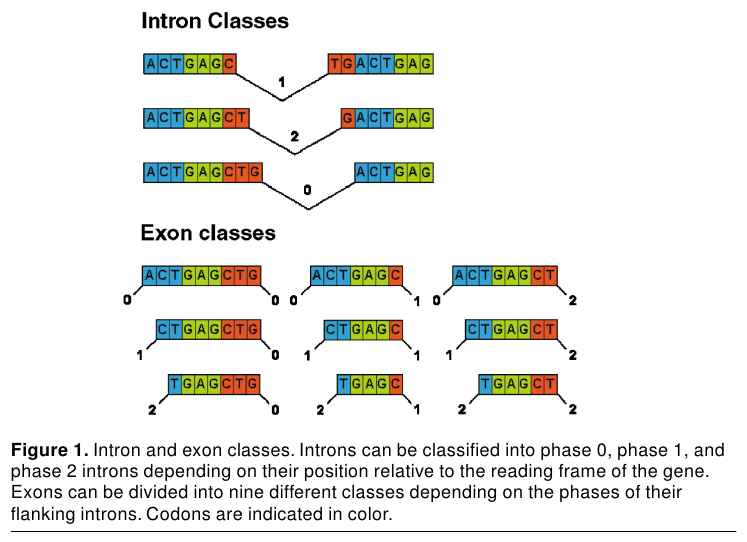
\includegraphics[scale=0.5]{kolkman-exon-2001-fig1}
    \caption{Kolkman (2001) Intron and exon phases \cite{kolkman_directed_2001}}
\end{figure}
\FloatBarrier

An interesting example of this is the Arabidopsis gene AT2G07815, which would
be classified as an orphan were it not for a short insert from an ancient
mitochondrial gene.


\subsection{Organelle Genes} Oddly, genomes sequencing projects often
ignore organelle genes. This may be a minor problem in metazoa, but in
plants can lead to serious issues. Including chloroplast and mitochondrial
genes, or at least specifying whether they were included, is vital in plant
phylostratigraphy.

\subsection{Proof of Transcription and Translation} Computational methods
provide some support, but orphans may sport particularly weak signals.
Transcription can be verified via RNA-Seq data. Ribosome foot-printing
evidence can be used as support of the orphans translatability (however
ribosome binding alone may not be sufficient to prove a transcript is
expressed \cite{guttman_ribosome_2013}).

\subsection{Database} More is not necessarily better. Find some paper on
this topic. Especially when masking is concerned. Also find a good example,
one of the BLINK things.

\subsection{Synteny and its usage in de novo classification}

Plant gene order is slowly shuffled, reviewed by Vision \cite{vision_gene_2005}.
